\newcommand\UniversiteAdi{Niğde Ömer Halisdemir Üniversitesi}
\newcommand\BolumAdi{MEKATRONİK BÖLÜMÜ}
\newcommand\DersKodu{MKT2002}
\newcommand\DersAdi{BİLGİSAYARLI KONTROL SİSTEMLERİ}
\newcommand\SinavAdi{Ödev 1}
\newcommand\SinavTarihi{10.03.2025}
\newcommand\SinavSaati{10:00}
\newcommand\SinavSuresi{90dk}

\pagestyle{fancy}
\fancyhf{} % clear existing header/footer entries
\fancyhead[R]{Öğrenci No:\hspace{4.5cm}}
\fancyhead[L]{Ad Soyad:\hspace{7cm}}
\noindent
\begin{tabular}{
    p{0.15\linewidth}
    p{0.15\linewidth}
    p{0.3\linewidth}
    p{0.1\linewidth}
    p{0.15\linewidth}}
    \multicolumn{5}{c}{\textbf{\BolumAdi}}\\
    \multicolumn{5}{c}{\textbf{\DersAdi}}\\\hline
    \multicolumn{1}{|r|}{Ders Kodu:}&
    \multicolumn{1}{|c|}{\DersKodu}&
    \multicolumn{1}{|c|}{}& 
    \multicolumn{1}{|r|}{Tarih:}&
    \multicolumn{1}{|c|}{\SinavTarihi} \\\hline
    \multicolumn{1}{|r|}{Sınav Türü:}&
    \multicolumn{1}{|c|}{\SinavAdi}&  
    \multicolumn{1}{|c|}{}&
    \multicolumn{1}{|r|}{Saat:}&
    \multicolumn{1}{|c|}{\SinavSaati}\\\hline
    \multicolumn{1}{|r|}{Dönemi:}&
    \multicolumn{1}{|c|}{2024-2025}&
    \multicolumn{1}{|c|}{}&
    \multicolumn{1}{|r|}{Süre:}&
    \multicolumn{1}{|c|}{\SinavSuresi} \\\hline
    &&&&\\
\end{tabular}\\\\
\noindent\begin{center}
\begin{tabular}{|r|c|}\hline
    &\textbf{Toplam}\\\hline
    \textbf{Puan:} &\textbf{100}\\\hline
    \textbf{Not:}  &\\\hline
\end{tabular}\end{center}
\noindent\textbf{Uyarı:}
\begin{itemize}\bfseries
    \item Soruları dikkatlice okuyunuz. Hesap makinesi kullanılabilir.
    \item İşlemleri atlamadan ve ayrıntılı olarak veriniz. Sadece nümerik yanıtlar veya çizimler ara işlemler olmadan kabul edilmemektedir.
    \item Yuvarlamalar 2 hane yapılacaktır. $\mathbf{1.99456\approx1.99}$ olarak alınacaktır.
\end{itemize}
\noindent\textbf{Soru:} Aktif süspansiyon sistemi için diferansiyel denklem 
\begin{equation}
\begin{split}
    m_1\frac{d^2x_1}{dt^2}&=-b_1\left(\frac{dx_1}{dt}-\frac{dx_2}{dt}\right)-k_1(x_1-x_2)+u\\
    m_2\frac{d^2x_2}{dt^2}&=b_2\left(\frac{dx_1}{dt}-\frac{dx_2}{dt}\right)+b_2\left(\frac{dw}{dt}-\frac{dx_2}{dt}\right)+k_2(w-x_2)-u
\end{split}
\end{equation}
olarak verilmiştir ve Şekil~\ref{fig:suspension} ile gösterilmektedir. Fark denklemlerini elde ediniz.
\begin{figure}[!htb]
    \centering
    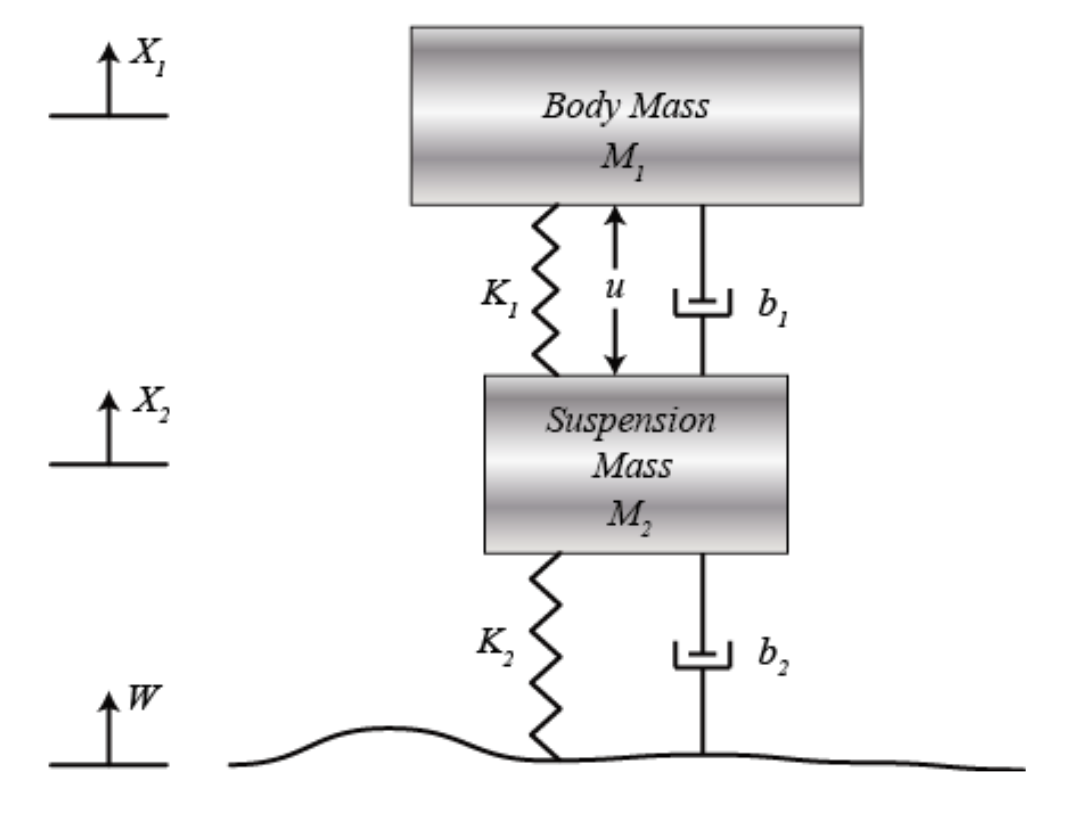
\includegraphics[width=0.8\textwidth]{suspension}
    \caption{Aktif süspansiyon sistemi modeli}\label{fig:suspension}
\end{figure}

\noindent\textbf{Çözüm:} 
Birinci dereceden türev
\begin{equation}
    \frac{dx}{dt}=\frac{x(k)-x(k-1)}{T}
\end{equation}
ve ikinci dereceden türev 
\begin{equation}
    \frac{d^2x}{dt^2}=\frac{x(k)-2x(k-1)+x(k-2)}{T^2}
\end{equation}
olarak ayrıklaştırılabilir. Bu durumda denklemler
\begin{equation}
\begin{split}
m_1\frac{x_1(k)-2x_1(k-1)+x_1(k-2)}{T^2}=-b_1\left(\frac{x_1(k)-x_1(k-1)}{T}-\frac{x_2(k)-x_2(k-1)}{T}\right)\\-k_1(x_1(k-2)-x_2(k-2))+u(k-2)\\
m_2\frac{x_2(k)-2x_2(k-1)+x_2(k-2)}{T^2}=b_2\left(\frac{x_1(k)-x_1(k-1)}{T}-\frac{x_2(k)-x_2(k-1)}{T}\right)\\+b_2\left(\frac{w(k)-w(k-1)}{T}-\frac{x_2(k)-x_2(k-1)}{T}\right)+k_2(w(k-2)-x_2(k-2))-u(k-2)
\end{split}
\end{equation}
ve
\begin{equation}
    \begin{split}
    m_1(x_1(k)-2x_1(k-1)+x_1(k-2))=-b_1T(x_1(k)-x_1(k-1)-x_2(k)+x_2(k-1))\\
    -k_1T^2(x_1(k-2)-x_2(k-2))+T^2u(k-2)\\
    m_2(x_2(k)-2x_2(k-1)+x_2(k-2))=b_2T(x_1(k)-x_1(k-1)-x_2(k)+x_2(k-1))\\
    +b_2T(w(k)-w(k-1)-x_2(k)+x_2(k-1))+k_2T^2(w(k-2)-x_2(k-2))-T^2u(k-2)
    \end{split}
\end{equation}
% \noindent\textbf{Extra:}Fark denklemlerini kullanarak $u$ girişine sıfır ve $w$ girişine birim basamak uygulayınız ve $x_1$ ve $x_2$ değişkenlerini çiziniz.
